%Random & 1 & 629.5462 & 282.9514 & 0.1368 & 0.0366 \\
%Saccadic & 1 & 98.8274 & 56.1298 & 0.1588 & 0.0370 \\
%Sweep & 1 & 601.5697 & 183.4529 & 0.1254 & 0.0454 \\
%$\epsilon$-Greedy & 1 & 112.9258 & 62.3798 & 0.1516 & 0.0398 \\


%\begin{landscape}
%\centering
%\vspace*{\fill}
\begin{table}[h!]
    \centering
    \begin{tabular}{| >{\centering} m{18mm} | >{\centering}m{22mm} | >{\centering}m{22mm} | >{\centering}m{22mm} | >{\centering}m{20mm} | m{20mm} <{\centering}|}
    \hline
       Strategy & Initial Belief Distribution & Mean TTD & Sample SD[TTD] & False Negative Rate & Proportion Incorrectly Localised \\
        \hline
        $\epsilon$-Greedy & Uniform & 112.9258 & 62.3798 & 0.1516 & 0.0398 \\
        $\epsilon$-Greedy & Gaussian & 21.68 & 20.44 & 0.0296 & 0.0118 \\
        \hline
        Sweep & Uniform & 601.5697 & 183.4529 & 0.1254 & 0.0454 \\
        Sweep & Gaussian & 464.48 & 185.54 & 0.0832 & 0.0294 \\
        \hline
        Saccadic & Uniform & 98.8274 & 56.1298 & 0.1588 & 0.0370 \\
        Saccadic & Gaussian & 14.558 & 18.75 & 0.0338 & 0.0114 \\
        \hline
        Random & Uniform & 629.5462 & 282.9514 & 0.1368 & 0.0366 \\
        Random & Gaussian & 501.83 & 268.45 & 0.0792 & 0.0308 \\
        \hline
    \end{tabular}
    \caption{Results of running the target localisation simulation with a Uniform initial belief distribution and Gaussian initial belief distribution for each implemented search strategy.}
    \label{table:VaryingPriorDistribution}
\end{table}
    
Table \ref{table:VaryingPriorDistribution} displays the results of running a simulation with a single agent and a single target while varying the initial belief distribution that the target is present in the search region. 
%The following parameters are fixed: Simulated Sensor False Negative Rate = 0.15, Simulated Sensor False Positive Rate = 0.2, Sensor model False Negative Rate = 0.15, Sensor Model False Positive Rate = 0.2, Initial belief that target is present in region = 0.5, SPRT Type \Romannum{1} error rate = 0.1, SPRT Type \Romannum{2} error rate = 0.15.
%\begin{itemize}
%    \item Simulated Sensor False Negative Rate = 0.15
%    \item Simulated Sensor False Positive Rate = 0.2
%    \item Sensor model False Negative Rate = 0.15
%    \item Sensor Model False Positive Rate = 0.2
%    \item Initial belief that target is present in region = 0.5
%    \item SPRT T\Romannum{1} error rate = 0.1, SPRT T\Romannum{2} error rate = 0.15.
%\end{itemize}
\begin{figure}
\centering
    \subfloat[Uniform initial belief distribution]{{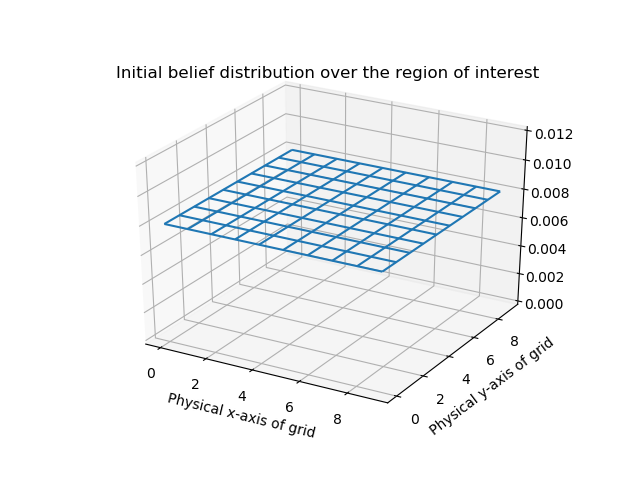
\includegraphics[width=6cm]{Chapters/MultiAgentTargetDetection/Figs/Results/Prior/Uniform/UniformInitialDistribution.png} }}%
    \qquad
    \subfloat[Gaussian initial belief distribution]{{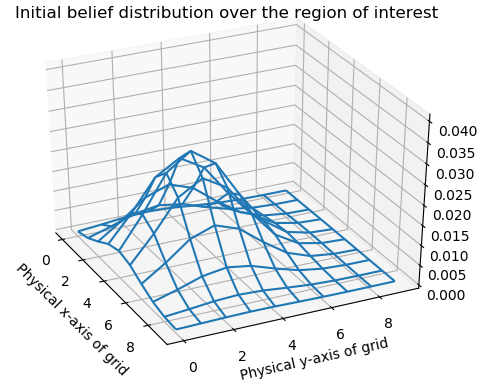
\includegraphics[width=6cm]{Chapters/MultiAgentTargetDetection/Figs/Results/Prior/Gaussian/GaussianInitialDistribution.png} }}%
    \caption{Initial belief distributions}%
    \label{fig:initialBeliefDistribution}%
\end{figure}
For each search strategy, we ran the simulation with both a Uniform and Gaussian initial belief distribution. The Gaussian mean coincided with the target location and the covariance matrix was $\begin{pmatrix} 3 & 0\\ 0 & 3\end{pmatrix}$, which is visualised in Figure \ref{fig:initialBeliefDistribution}. This represents a correct suspicion about the location of the target, which is the case in scenarios where some prior information may suggest clues to the target location. As expected, for all of the search strategies the expected time until a decision reduces dramatically when using the Gaussian prior relative to the Uniform prior. 
%In the case of the two non-adaptive search methods (random and sweep), the effect is lessened as the search process is not influenced by new observations. 
Since the shape of the Gaussian distribution is aligned more closely to the true distribution that the Uniform distribution, it takes fewer samples to reach a sufficiently peaked distribution to reach the acceptance region for the SPRT. 
%This is visible by examining the evolution of the cumulative agent belief that the target is present in the region, shown in figures x and y.

\par It can also be seen that the false negative rate (the rate at which the agent incorrectly concludes that the target is not present in the region) drops in the case of the Gaussian prior relative to the Uniform prior. This is also a result of using a prior distribution that matches the shape of the true distribution, since it requires a significant number of false positive/negative samples to modify the distribution enough to reach a negative conclusion.

%This is due to the unbiased sampling method of the non-adaptive strategies, which 

%but is higher for the non-adaptive search strategies since they are unbiased while sampling grid locations.
   

%    \hline
%    \multicolumn{2}{c}{Initial Discretised Gaussian Distribution of Belief Over Grid Cells (random mean, covariance matrix = [[], []]}\\
%    \hline

%\textbf{Gaussian Initial Belief Distribution (Mean coinciding with true target location)}
%\begin{table}[h!]
%    \centering
%    \begin{tabular}{| >{\centering} m{18mm} | >{\centering}m{20mm} | >{\centering}m{18mm} | >{\centering}m{20mm} | >{\centering}m{20mm} | m{20mm} <{\centering}|}
%    \hline
%       Strategy & Initial Belief Distribution & E[Time To Decision] & SD[Time To Decision] & False Negative Rate & Proportion Incorrect Localised \\
%        \hline
%        $\epsilon$ -Greedy & Gaussian & 21.68 & 20.44 & 0.0296 & 0.0118 \\
%        Sweep & Gaussian & 464.48 & 185.54 & 0.0832 & 0.0294 \\
%        Saccadic & Gaussian & 14.558 & 18.75 & 0.0338 & 0.0114 \\
%        Random & Gaussian & 501.83 & 268.45 & 0.0792 & 0.0308 \\
%    \hline
%    \end{tabular}

%  \caption{Results of running the target localisation simulation with a  uniform initial belief distribution and Gaussian initial belief distribution. p(T \Romannum{1}) = The probability of making a type \Romannum{1} error using the SPRT, p(T \Romannum{2}) = The probability of making a type \Romannum{1} error using the SPRT, Sim. FPR = The simulated false positive rate of the sensor, Sim. FNR = The simulated false negative rate of the sensor, E[TTD] = The expected amount of timesteps until a decision is made, Prec. = precision, Rec. = Recall. }\label{table:PriorGaussian}
%\end{table}





%\begin{landscape}

%\end{landscape}


































